% DigitaltechnikFS										Stand: 08.02.2019
% Digitaltechnik Formelsammlung für WiSe 2018/2019			
% 8 Seiten
% Dokumenteinstellungen
% ======================================================================

% Dokumentklasse (Schriftgröße 6, DIN A4, Artikel)
\documentclass[6pt,a4paper]{scrartcl}

% Seitenlayout und Ränder:
\usepackage{geometry}
\geometry{a4paper,landscape, left=6mm,right=6mm, top=0mm, bottom=3mm,includeheadfoot} 

% Dokumentbeschreibung
\title{Digitaltechnik Formelsammlung}
\author{Emanuel Regnath, Martin Zellner, Hendrik Böttcher}

% Pakete laden
\usepackage[utf8x]{inputenc}	% Zeichenkodierung: UTF-8 (für Umlaute)   
\usepackage[german]{babel}		% Deutsche Sprache
\usepackage{multicol}			% Spaltenpaket
\usepackage{amsmath}			% Mathematische Formelzeichen
\usepackage{amssymb}			% Mathematische Formelzeichen
\usepackage{esint}				% erweiterte Integralsymbole
\usepackage{multicol}			% ermöglicht Seitenspalten  
\usepackage{booktabs}			% bessere Tabellenlinien
\usepackage{color}				% Farben
\usepackage{colortbl}			% für die Hintergrundfarbe einzelner Zellen in Tabellen
\usepackage{graphicx}			% Grafiken
\usepackage{pbox}				% Intelligent parbox: \pbox{maximum width}{blabalbalb \\ blabal}
%\usepackage{undertilde}			% Tilde unter Zeichen
\newcommand{\utilde}[1]{#1}
\usepackage{scrtime}			% Uhrzeit

%Farben
\definecolor{lightgray}{rgb}{0.8,0.8,0.8}
\definecolor{gray}{rgb}{0.9,0.9,0.9}

%Kopf- und Fußzeile
\usepackage{fancyhdr}
\pagestyle{fancy}
\fancyhf{}

   \fancyfoot[C]{Emanuel Regnath (Emanuel.Regnath@tum.de), Martin Zellner (martin.zellner@mytum.de), Hendrik Böttcher (hendrik.boettcher@tum.de)}
   \renewcommand{\headrulewidth}{0.0pt} %obere Linie ausblenden
   \renewcommand{\footrulewidth}{0.1pt} %obere Linie ausblenden
   \fancyfoot[R]{(Gekürzt, überarbeitet - lukas.kompatscher@tum.de) Stand: \todayV \qquad \thepage}
   \fancyfoot[L]{Homepage: www.latex4ei.de -  Fehler bitte \emph{sofort} melden.}
	
% Schriftart SANS für bessere Lesbarkeit bei kleiner Schrift
\renewcommand{\familydefault}{\sfdefault} 
\renewcommand{\emph}[1]{\textsf{\textbf{#1}}}

% Array- und Tabellenabstände vergrößern
\renewcommand{\arraystretch}{1.2}
\renewcommand{\vec}[1]{\ensuremath{\underline{\boldsymbol {#1}}}}


% Eigene Befehle
\newcommand{\todayV}{\the\day.\the\month.\the\year}                     	    	% Datum D.M.YYYY
\newcommand{\iset}[2]{\ensuremath{\bigl\{ \bigl. #1 \, \bigr| \, #2 \bigr\}}}		% intensional set
\newcommand{\eset}[1]{\ensuremath{\bigl\{#1\bigr\}}}								% extensional set
\newcommand{\norm}[1]{\ensuremath{\|#1\|}}											% Norm
\newcommand{\gk}[1]{\ensuremath{\left\lfloor#1\right\rfloor}} 						% Gaußklammer
\newcommand{\sprod}[2]{\ensuremath{\left\langle #1, #2 \right\rangle }}				% Skalarprodukt
\newcommand{\abs}[1]{\ensuremath{\left\vert#1\right\vert}} 							% Betrag
\newcommand{\mat}[1]{\ensuremath{\begin{bmatrix} #1 \end{bmatrix}}}					% Matrix
\newcommand{\vect}[1]{\ensuremath{\begin{pmatrix} #1 \end{pmatrix}}}				% Vektor
\newcommand{\mvect}[1]{\ensuremath{\left. \begin{matrix} #1 \end{matrix}  \right]}} % Matrixvektor
\newcommand{\ma}[1]{\ensuremath{\utilde{\bs {#1}}}}

% Abkürzungen
\newcommand{\ul}[1]{\ensuremath{\underline{#1}}}								%Untersteichen
\newcommand{\ol}[1]{\ensuremath{\overline{#1}}}									%Überstreichen
\newcommand{\Ra}[0]{\ensuremath{\Rightarrow}}									%Rightarrow
\newcommand{\ra}[0]{\ensuremath{\rightarrow}} 									%Rightarrow
\newcommand{\n}[0]{\ensuremath{\overline}}										%NOT
\newcommand{\bs}[1]{\ensuremath{\boldsymbol{#1}}}								%Fett und kursiv im mathmode
\newcommand{\diff}{\ensuremath{\ \mathrm d}}									%delta
\newcommand{\grad}{\ensuremath{\mathrm{grad}\ }}								%Gradient
\renewcommand{\div}{\ensuremath{\mathrm{div}\ }}								%Divergenz
\newcommand{\rot}{\ensuremath{\mathrm{rot}\ }}									%Rotation
\newcommand{\Sp}{\ensuremath{\mathrm{Sp}\ }}									%Spur
	% Für Mengen
	\newcommand{\N}{\ensuremath{\mathbb N}}
	\newcommand{\R}{\ensuremath{\mathbb R}}
	\newcommand{\C}{\ensuremath{\mathbb C}}

%Überschreibungen
\renewcommand{\arraystretch}{1.2}
\renewcommand{\vec}[1]{\ensuremath{\underline{\boldsymbol {#1}}}}
\newcommand{\imglog}{\includegraphics[width=.85cm]}


% Dokumentbeginn
% ======================================================================

\begin{document}


% Aufteilung in Spalten
\begin{multicols*}{3}

% -------------------------------------------
% | 		Digitaltechik					|
% ~~~~~~~~~~~~~~~~~~~~~~~~~~~~~~~~~~~~~~~~~~~
%=======================================================================
\parbox{2.3cm}{
	
\includegraphics[height=2cm]{img/Logo.pdf}
}
\parbox{4cm}{
	\emph{\huge{Digitaltechnik}}
}

% ======================================================================
\section{Moore'sches Gesetz}
\begin{itemize} \itemsep0pt
	\item alle 18-24 Monate verdoppelt sich die Anzahl der Transistoren auf gleicher Fläche
	\item Exponentielles Wachstum der Transistorzahl, exponentieller Rückgange des Preises pro Transistor
	\item Herstellungskosten (Fixkosten, Variable Kosten, Technologiefaktor), Entwicklerproduktivität, Verlustleistungsdichte
\end{itemize}

\section{Einheiten}
\begin{multicols}{3}
\begin{tabular}{c | c}
	Potenz & Vorsatz \\ \midrule
	$10^{12}$ & T \\
	$10^{9}$ & G \\
	$10^{6}$ & M \\
	$10^{3}$ & k \\
	$10^{2}$ & h \\
	$10^{1}$ & da 
\end{tabular}
\begin{tabular}{c | c}
	Potenz & Vorsatz \\ \midrule
	$10^{-1}$ & d \\
	$10^{-2}$ & c \\
	$10^{-3}$ & m \\
	$10^{-6}$ & $\mu$	\\
	$10^{-9}$ & n \\
	$10^{-12}$ & p \\
	$10^{-15}$ & f
\end{tabular}
\begin{tabular}{ r | l }
$Hz$ & $s^{-1}$ \\
N & $kg m s^{-2} $ \\
$J $ & $ N m = V A s$\\
$W $ & $ V A  = J s^{-1} $ \\
$ C $ & $ A s $ \\
$V $ & $ J C^{-1} $\\
$F $ & $ C V^{-1} $ \\
$\Omega $ & $ V A^{-1} $\\
$ H $ & $ V s  A^{-1}$
\end{tabular}
\end{multicols}
$Bit \xrightarrow{\cdot 8} Byte \xrightarrow{\cdot 1024} kByte \xrightarrow{\cdot 1024} MByte$\\
	
\section{Boolsche Algebra}

	\subsection{Boolesche Operatoren (Wahrheitstabelle WT)}
	\begin{tabular}{c|c!{\vrule width 1pt}c|c|c|c|c|c}
		& & \imglog{img/logic/and-us.png} & \imglog{img/logic/or-us.png} & \imglog{img/logic/xor-us.png} & \imglog{img/logic/nand-us.png} & \imglog{img/logic/nor-us.png} & \imglog{img/logic/xnor-us.png} \\
		& & \imglog{img/logic/and-din.png} & \imglog{img/logic/or-din.png} & \imglog{img/logic/xor-din.png} & \imglog{img/logic/nand-din.png} & \imglog{img/logic/nor-din.png} & \imglog{img/logic/xnor-din.png} \\
		& & \imglog{img/logic/and-iec.png} & \imglog{img/logic/or-iec.png} & \imglog{img/logic/xor-iec.png} & \imglog{img/logic/nand-iec.png} & \imglog{img/logic/nor-iec.png} & \imglog{img/logic/xnor-iec.png} \\
		x & y &    AND     &  OR   &     XOR     &         NAND          &       NOR        &          EQV           \\
		  &   & $x\cdot y$ & $x+y$ & $x\oplus y$ & $\overline{x\cdot y}$ & $\overline{x+y}$ & $\overline{x\oplus y}$ \\ \hline\hline
		0 & 0 &     0      &   0   &      0      &           1           &        1         &           1            \\ \hline
		0 & 1 &     0      &   1   &      1      &           1           &        0         &           0            \\ \hline
		1 & 0 &     0      &   1   &      1      &           1           &        0         &           0            \\ \hline
		1 & 1 &     1      &   1   &      0      &           0           &        0         &           1
	\end{tabular}
	Konfiguration: $f = c_1 + c_2 + c_3 \Ra cov(f) = \eset{c_1, c_2, c_3}$

	\subsection{Gesetze der booleschen Algebra}
	\begin{tabular}{l|l|l}
		            & Boolesche Algebra                                     & Mengenalgebra                                         \\
		            & $({0,1};\cdot , +, \overline{x})$                     & $(P(G);\cap , \cup, \overline{A};G,\emptyset )$       \\ \hline
		Kommutativ  & $x \cdot y = y \cdot x$                               & $A \cap B = B \cap A$                                 \\
		            & $x + y = y + x$                                       & $A \cup B = B \cup A$                                 \\
		Assoziativ  & $x \cdot (y \cdot z) = (x \cdot y) \cdot z$           & $(A \cap B) \cap C = A \cap (B \cap C)$               \\
		            & $x + (y + z) = (x + y) + z$                           & $(A \cup B) \cup C = A \cap (B \cup C)$               \\
		Distributiv & $x \cdot (y + z) = x \cdot y + x \cdot z$             & $A \cap (B \cup C) = (A \cap B) \cup (A \cap C)$      \\
		            & $x + (y \cdot z) = (x + y) \cdot (x + z)$             & $A \cup (B \cap C) = (A \cup B) \cap (A \cup C)$      \\
		Indempotenz & $x \cdot x = x$                                       & $A \cap A = A$                                        \\
		            & $x + x = x$                                           & $A \cup A = A$                                        \\
		Absorbtion  & $x \cdot (x+y) = x$                                   & $A \cap (A \cup B) = A$                               \\
		            & $x + (x \cdot y) = x$                                 & $A \cup (A \cap B) = A$                               \\
		Neutral     & $x \cdot 1 = x$                                       & $A \cap G = A$                                        \\
		            & $x + 0 = x$                                           & $A \cup \emptyset = A$                                \\
		Dominant    & $x \cdot 0 = 0$                                       & $A \cap \emptyset = \emptyset$                        \\
		            & $x + 1 = 1$                                           & $A \cup G = G$                                        \\
		Komplement  & $x \cdot \overline{x} = 0$                            & $A \cap \overline{A} = \emptyset$                     \\
		            & $x + \overline{x} = 1$                                & $A \cup \overline{A} = G$                             \\
		            & $\overline{\overline{x}} = x$                         & $\overline{\overline{A}} = A$                         \\
		De Morgan   & $\overline{x \cdot y} = \overline{x} + \overline{y}$  & $\overline{A \cap B} = \overline{A} \cup \overline{B}$\\
		            & $\overline{x + y} = \overline{x} \cdot \overline{y}$ & $\overline{A \cup B} = \overline{A} \cap \overline{B}$
	\end{tabular}


	\subsection{Boolesche Funktionen}	
	\begin{equation*}
	f:\{0,1\}^n\ra \{0,1\} \qquad \qquad f(\vec{x})=f(x_1,x_2,\dots,x_n) 
	\end{equation*} \\
	Einsmenge $F$ von $f$: $F=\{\vec{x}\in \{0,1\}^n|f(\vec{x})=1\}$ \\
	Nullmenge $\overline F$ von $f$: $\overline F=\{\vec{x}\in \{0,1\}^n|f(\vec{x})=0\}$
	\paragraph{Kofaktor bezüglich}
	\begin{itemize}\itemsep0pt
	\item $x_i: f_{x_i}=f|_{x_i=1}=f(x_1,\dots,1,\dots,x_n)$
	\item $\overline x_i: f_{\overline x_i}=f|_{x_i=0}=f(x_1,\dots,0,\dots,x_n)$
	\end{itemize}
	\paragraph{Eigenschaften von $f(\vec{x})$}
	\begin{itemize}\itemsep0pt
		\item tautologisch $\Leftrightarrow f(\vec{x})=1 \qquad \forall \vec x \in \{0,1\}^n$
		\item tautologisch $\Leftrightarrow f(\vec{x})=1 \qquad \forall \vec x \in \{0,1\}^n$
		\item kontradiktorisch $\Leftrightarrow f(\vec{x})=0 \qquad \forall \vec x \in \{0,1\}^n$
				\item unabhängig von $x_i \Leftrightarrow f_{x_i} = f_{\overline x_i}$
						\item abhängig von $x_i \Leftrightarrow f_{x_i} \ne f_{\overline x_i}$
			\end{itemize}
	
	\subsection{Multiplexer}
	\begin{tabular}{ll}
		$f = x \cdot a + \overline x \cdot b$ & (2 Eingänge $a,b$ und 1 Steuereingang $x$)\\
		$f = \ol x_1 \ol x_2 a + \ol x_1 x_2 b + x_1  \ol x_2 c + x_1 x_2d$ & (Eingänge: $a,b,c,d$  Steuerung: $x_1$, $x_2$)\\
	\end{tabular}



	\subsection{Wichtige Begriffe}
	\begin{tabular}{l|l|l}
		Wichtige Begriffe: & Definition & Bemerkung\\ \hline
		Signalvariable & $x$ & $\hat x \in \eset{0,1}$ \\
		Literal & $l_i = x_i$ oder $\overline{x_i}$ & $i \in I_0=\eset{1,...,n}$\\
		Minterme,0-Kuben & M0C $\ni m_j = \prod\limits_{i\in I_0} l_i$ & $|$M0C$| = 2^n$ \\
		d-Kuben & MC $\ni c_j = \prod\limits_{i\in I_j \subseteq I_0} l_i$ & $|$MC$|=3^n$\\
		Distanz & $\delta(c_i,c_j) = \bigl| \iset{l}{l \in c_i \land \overline{l}\in c_j}  \bigr|$ & $\delta_{ij} = \delta(c_i,c_j)$ \\
		Implikanten & $MI = \iset{c \in MC}{c \subseteq f}$ &  \\
		Primimplikanten & $MPI = \iset{p \in MI}{p \not\subset c \ \forall c \in MI}$ & $MPI \subseteq MI \subseteq MC$\\
	\end{tabular}\\ \\ \\
	\begin{tabular}{l|l|l}	
		SOP (DNF) & eine Summe von Produkttermen & Terme sind ODER-verknüpft \\
		POS (KNF) & ein Produkt von Summentermen & Terme sind UND-verknüpft\\
		CSOP (KDNF)& Summe aller Minterme & WT: 1-Zeilen sind Minterme\\
		CPOS (KKNF)& Menge aller Maxterme & WT: 0-Zeilen negiert sind Maxterme \\
		VollSOP (nur 1)& Menge aller Primimplikanten & Bestimmung siehe Quine Methode\\
		& & oder Schichtenalgorithmus\\
		MinSOP (min. 1)& Minimale Summe v. Primimplikanten & durch Überdeckungstabelle \\
	\end{tabular}
	\\ \\
	FPGA: Field Programmable Gate Array\\
	LUT: Look Up Table\\




\section{Beschreibungsformen}
	\subsection{Disjunktive Normalform/Sum of products (DNF/SOP)}
	\textbf{Eins-Zeilen} als \textbf{Implikanten} (UND) schreiben und alle Implikanten mit \textbf{ODER} verknüpfen: \\
	$Z = \overline A \cdot \overline B + \overline C \cdot D$ 
	
	\subsection{Konjunktive Normalform/Product of sums (KNF/POS)}
	\textbf{Null-Zeilen negiert als Implikat} (ODER)  schreiben und alle Implikaten \textbf{UND} verknüpfen: \\	
	$Z = ( \ol A + \ol C) \cdot ( \ol A + \ol D) \cdot ( \ol B + \ol C) \cdot ( \ol B + D)$
	
	\subsection{Umwandlung in jeweils andere Form}
	1. Doppeltes Negieren der Funktion: $ Z = \overline {\overline{\overline A \cdot \overline B + \overline C \cdot D}}$\\
	2. Umformung "'untere"'  Negation (DeMorgan) : $ Z = \ol{\ol{\ol A \cdot \ol B} \cdot \ol{\ol C \cdot D}} = \ol{(A+B) \cdot (C+\ol D)}$\\
	3. Ausmultiplizieren: $ Z = \ol{(A+B) \cdot (C+\ol D)} = \ol{A\cdot C + A\cdot \ol D + B \cdot C + B \cdot \ol D}$\\
	4. Umformung "'obere"'  Negation (DeMorgan) :\\ $ Z= \ol{AC} \cdot \ol{A \ol D} \cdot \ol{BC} \cdot \ol{B\ol D} = ( \ol A + \ol C) \cdot ( \ol A + D) \cdot ( \ol B + \ol C) \cdot ( \ol B + D)$\\ \\
	Analog von KNF (POS) nach DNF (SOP).
	
\section{Logikminimierung}
	\subsection{Nomenklatur}
	\begin{itemize}\itemsep0pt
	\item $m_i$ Minterm: UND-Term in dem alle Variablen vorkommen (aus KDNF)
	\item $M_i$ Maxterm: ODER-Term in dem alle Variablen vorkommen (aus KKNF)
	\item $c_i$ Implikant: UND-Term in dem freie Variablen vorkommen können
	\item $C_i$ Implikat: ODER-Term in dem freie Variablen vorkommen können
	\item $p_i$ Primimplikant: UND-Term mit maximal freien Variablen
	\item $P_i$ Primimplikat: ODER-Term mit maximal freien Variablen
	\end{itemize}

	\subsection{Karnaugh-Diagramm} % (fold)
	\textbf{Vorteile}: sehr anschaulich\\
	\textbf{Nachteile}: Gray-Kodierung notwendig, nur wenige Inputvariablen\\
		Zyklische Gray-Codierung: 2dim:$00,01,11,10$ 3dim:$000,001,011,010,110,111,101,100$
		
	\begin{tabular}{l | c | c |  c | r}
	$_z\!\!\diagdown \!\!^{xy}$ & 00 	& 	01	&	11 	&	10	 	\\ \midrule
	0		&	1 \cellcolor{gray}	&	0	&	0	&	0		\\	
	1		&	X \cellcolor{gray}	&	1 \cellcolor{lightgray}	&	1 \cellcolor{lightgray}	&	0		\\	
	\end{tabular}
	Gleiche Zellen zusammenfassen: z.B. $\overline x \overline y + y \cdot z$\\
	Don't Care Werte ausnutzen!
	% subsection Karnaugh- Diagramm (end)

	\subsection{Quine Methode}
	\textbf{Vorteile}: automatisierbar (DEA/FSM), beliebig viele Inputvariablen\\
	\textbf{Nachteile}: viele paarweise Vergleiche, Erweiterung auf KKNF oder KDNF notwendig, viele Min- und Maxterme\\
	geg.: DNF/KNF oder Wertetabelle von $f(x)$ \\
	ges.: alle Primimplikanten $p_i$ (VollSOP)  \\ \\
	Spezielles Resoltuionsgesetz: $x\cdot a + \overline x \cdot a = a$ \\
	Absorptionsgesetz: $a + a\cdot b = a$
	
	\begin{enumerate}
		\item kanonische Form (KKNF/KDNF) bestimmen (z.B. $f(x,y,z) = xy = xyz + xy\overline z$)
		\item Alle Min-/Maxterme in Tabelle eintragen (Index von m ist (binär)Wert des Min-/Maxterms), sortieren nach der Anzahl der negierten Literale (=Klasse)
		\item 1-Kubus: Minterme die sich um eine Negation unterscheiden, zu einem Term verschmelzen (Resolutionsgesetz), dabei notieren aus welchen 0-Kuben er besteht und alle verwendeten 0-Kuben abhaken
		\item Der 1-Kubus muss zusammenhängend sein! (d.h. alle 1-Kubus Minterme müssen zusammenhängen)
		\item Wenn möglich 2-Kubus bilden.
		\item Wenn keine Kubenbildung mehr möglich $\ra$ Nicht abgehakte Kuben sind Primimplikanten
	\end{enumerate}
	Beispiel (Quine Methode):
	
	\begin{tabular}{l | c | c  || c | c | c || c | c | r}
	      & 0-Kubus & A & 1-Kubus & R & A & 2-Kubus  & A \\
	$m_1$ & $\overline x_1 \overline x_2 x_3$ & $\surd$ & $\overline x_2 x_3$ & $m_1 \& m_5$ & $p_1$ & &\\
	$m_4$ & $x_1 \overline x_2 \overline x_3$ & $\surd$ & $x_1 \overline x_2$ & $m_4 \& m_5$ & $\surd$ & $x_1$ &   $p_2$\\
	$m_5$ & $x_1 \overline x_2  x_3$ & $\surd$  & $x_1 \overline x_3$ & $m_4 \& m_6$ & $\surd$& &\\
	$m_6$ & $x_1 x_2 \overline x_3$ & $ \surd$ & $x_1 x_3$ & $ m_5 \& m_7$ & $ \surd$ & &\\
	$m_7$ & $x_1 x_2 x_3$ & $\surd$ & $x_1 x_2$ & $m_6 \& m_7 $ & $ \surd$ & &\\
	\end{tabular} \\ \\
	$\Ra f(x_1,x_2,x_3)=p_1+p_2=\ol x_2x_3 + x_1$
	
	\subsection{Resolventenmethode} % (fold)
	\label{sec:Resolventenmethode}
		\textbf{Vorteile}: Keine KDNF Notwendig, skaliert für viele Inputvariablen\\
		Ziel: alle Primimplikanten \\ \\
		Wende folgende Gesetze an: \\
		Absorptionsgesetz: $a + ab = a$ \\
		allgemeines Resolutionsgesetz: $x \cdot a + \overline x \cdot b = x \cdot a + \overline x \cdot b + ab$ \\
		\\
		Anwendung mit Schichtenalgorithmus
		\begin{enumerate}
			\item schreibe die Funktion $f$ in die 0. Schicht
			\item bilde \textbf{alle möglichen} Resolventen aus der 0. Schicht und schreibe sie in die nächste Schicht als ODER Verknüpfungen (Resolventen zu $f$ "hinzufügen")
			\item überprüfe ob Resolventen aus der 1. Schicht Kuben aus Schicht 0 überdecken(Absorbtion) und streiche diese Kuben aus Schicht 0
			\item Schicht i besteht aus den möglichen Resolventen von Schicht 0 bis $(i-1)$. Abgestrichene Kuben aus vorherigen Schichten brauchen \textbf{nicht} mehr beachtet werden.
			\item Sobald in der i-ten Schicht +1 steht oder keine weiteren Resolventen gebildet werden können, ist man fertig. 
			$\Ra $ alle nicht ausgestrichenen Terme bilden die VollSOP
		\end{enumerate}
		
		\begin{tabular}{l | r}
		$f(x_1, \ldots, x_n)$ & Schicht \\ \midrule
		$x \cdot w + \overline x \cdot w + x \cdot y \cdot w \cdot \overline z + \overline x \cdot y \cdot w \cdot \overline z + \overline y \cdot w \cdot \overline z $& $0$ \\
		$+ w + y \cdot w \cdot \overline z$ & $1$ \\
		$+ w \cdot \overline z $ & $2$ \\
		$+ w$ &$ 3$
		\end{tabular}
	% section Resolventenmethode (end)

	\subsection{Überlagerung Bestimmung der MinSOP}
	Geg: CSOP/KDNF ($\sum m_i$) und VollSOP ($\sum p_i$) \qquad Ges: MinSOP (Minimalform)\\
	Überdeckung: $\begin{array}{rccl} C = & (m_0 \subseteq p_1) & \cdot (m_2 \subseteq p_1 + m_2 \subseteq p_2) & \stackrel{!}=1 \\ C = & \tau_1 & \cdot (\tau_1 + \tau_2) & = \tau_1 + \tau_1 \tau_2 = \tau_1 \end{array}$ \\
	Alternativ: Mit Überdeckungstabelle bestimmen. Bsp:\\
	\begin{tabular}{|c|c|c|c|c|c|}
		\hline
		          &      \multicolumn{4}{c|}{Minterme}  &      \\ \hline
		Primterme &  $m_1$  &  $m_2$  & \dots &  $m_N$  & $L(p_i)$   \\ \bottomrule[1pt]
		  $p_1$   & $\surd$ &         &       &         & $L(p_1)$   \\ \hline
		  $p_2$   & $\surd$ &         &       & $\surd$ & $L(p_2)$   \\ \hline
		 \vdots   &         &         &       &         &  \vdots    \\ \hline
		  $p_K$   &         & $\surd$ &       &         & $L(p_K)$   \\ \hline
	\end{tabular} \\
	$K$: Anzahl der Primterme\\
	$N$: Anzahl der Minterme \\
	$L(p_i)$: Kosten/Länge der Primimplikanten\\
	\textbf{Vorgehen}: erst alle \textbf{überdeckenden} Spalten, dann alle \textbf{überdeckten} Zeilen streichen.
	
\section{Halbleiter}
\begin{tabular}{l|c|c|c|c|c}
	& Isolator & Metall & undotiert & N-Typ & P-Typ \\ \hline
	Ladungsträger & Keine & $e^-$ & $e^- / e^+$ & $e^-$ & $e^+$ \\
	Leitfähigkeit & Keine & Sehr hoch & $\propto T$ & Hoch & Mittel\\  
\end{tabular}

\section{MOS-FET's}
% ======================================================================
\textbf{M}etal \textbf{O}xide \textbf{S}emiconductor \textbf{F}ield \textbf{E}ffekt \textbf{T}ransistor\\
\parbox{4.0cm}{ 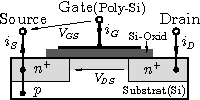
\includegraphics{img/ds/mosfet.pdf} \\ $V_{Pinch-Off} = V_{GS} - V_{th}$ } \parbox{3.0cm}{ 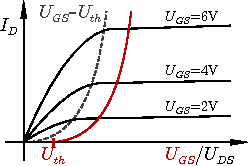
\includegraphics{img/ds/char_nmos.pdf} } 


	\subsection{Bauteilparameter}
	Verstärkung: \framebox{
			$\beta = K' \frac{W}{L} \text{ mit } K' = \frac{\mu \varepsilon_{ox} \varepsilon_0}{t_{0x}} \qquad [\beta]=\frac{A}{V^2}$ 
		} \\
	\begin{tabular} {r | l}
		Kanalweite & W  \\
		Kanallänge & L  \\
		Elektronenbeweglichkeit & $\mu$\quad $\mu_n \approx 250 \cdot 10^{-4} \frac{m^2}{Vs}$, $\mu_p \approx 100 \cdot 10^{-4} \frac{m^2}{Vs}$ \\
		rel. Dielektrizität des Gateoxyds & $\varepsilon_{ox} \approx 3,9$ \\
		Dielektrizitätskonstante & $\varepsilon_0 = 8.8541878 \cdot 10^{-12} \frac{\mathrm{A\,s}}{\mathrm{V\,m}}$ \\
		Gateoxyddicke & $t_{ox}$ \\
		Verstärkung & $\beta = \frac{\mu_n \varepsilon_{ox} \varepsilon_0}{t_{ox}} \cdot \frac{W}{L} = K' \frac{W}{L} = \frac{\mu_n C_G}{L^2}$ \\
		Kapazität & $C_G = \varepsilon_{ox} \varepsilon_0 \frac{WL}{t_{ox}}$ \\
		Verzögerungszeit & $t_{pHL} \propto \frac{C_L t_{ox} L_p}{W_p \mu_p \varepsilon_{ox} (V_{DD} - |V_{th}|)}$ \\
	\end{tabular}
	\begin{itemize}
		\item große Kanalweite $\Ra$ große Drain-Störme \\ $\Ra$ schnelle Schaltgeschwindigkeit (da $i_d \propto \beta \propto \frac{W}{L}$) \\
		Aber: große Fläche.
		\item nMos schaltet schneller als pMOS, da nMOS und pMOS unterschiedliche Majoritätsladungsträger haben. Die Beweglichkeit der Löcher ist im Allgemeinen geringer als die der Elektronen. 
	\end{itemize}
	
	\subsection{Drainstrom}
		\textbf{nMos} (p-dotiertes Substrat, n-dotierte Drain/Source), schlechter pull up (Pegeldegenerierung)
		\begin{equation*}
		\!\!\! I_d = \begin{cases}
		0, &\text{ für }  U_{gs} - U_{th} \le 0 \qquad \qquad  \text{(Sperrber.)}\\[0.2em]
		 \beta [(u_{gs} - U_{th}) \cdot u_{ds} - \frac{1}{2} u_{ds}^2] , &\text{ für }  0 \le U_{gs} - U_{th} \ge u_{ds} \  \text{(linearer Ber.)}\\\\[0.2em]
		 \frac{1}{2} \beta \cdot (u_{gs} - U_{th})^2, &\text{ für }  0 \le U_{gs} - U_{th} \le u_{ds} \  \text{(Sättigungsber.)}\\
		\end{cases}
		\end{equation*}
		\textbf{pMos} (n-dotiertes Substrat, p-dotierte Drain/Source), schlechter pull down (Pegeldegenerierung)
		\begin{equation*}
		\!\!\! I_d = \begin{cases}
		0, &\text{ für }  U_{gs} - U_{th} \ge 0 \qquad \qquad  \text{(Sperrber.)}\\[0.2em]
		- \beta [(u_{gs} - U_{th}) \cdot u_{ds} - \frac{1}{2} u_{ds}^2] , &\text{ für }  0 \ge U_{gs} - U_{th} \le u_{ds} \  \text{(linearer Ber.)}\\\\[0.2em]
		- \frac{1}{2} \beta \cdot (u_{gs} - U_{th})^2, &\text{ für }  0 \ge U_{gs} - U_{th} \ge u_{ds} \  \text{(Sättigungsber.)}\\
	
		\end{cases}
		\end{equation*}

	
	\subsection{pMos und nMos}
	\pbox{3.0cm}{ 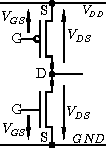
\includegraphics{img/ds/cmos.pdf} } 
	\pbox{10.0cm}{
	\begin{tabular}{c|c|c|c}
		Transistor & Source liegt immer am & $V_{GS},V_{DS},I_D$ & Substrat \\ \midrule
		$\underset{\text{normally on}}{\text{pMos}}$ & höheren Potential & $\bs{< 0}$ & $+(V_{DD})$ \\
		& & & \\
		& & & \\
		$\underset{\text{normally off}}{\text{nMos}}$ & niedrigeren Potential & $\bs{> 0}$ & $-(GND)$ \\
	\end{tabular}\\[0.5cm]
	}
	
\section{CMOS - Logik}
% ======================================================================
	\emph{Vorteil:}	 (Fast) nur bei Schaltvorgängen Verlustleistung - wenig statische Verluste \\
Drei Grundgatter der CMOS-Technologie:\\
	\begin{tabular}{ccc}
		NOT (2 Trans.) & NAND (4 Trans.) & NOR (4 Trans.)\\
		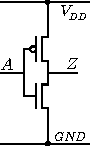
\includegraphics{img/ds/mosfet_not.pdf} \qquad & 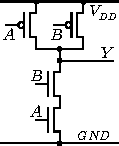
\includegraphics{img/ds/mosfet_nand.pdf} \qquad & 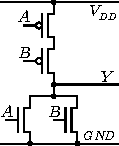
\includegraphics{img/ds/mosfet_nor.pdf} \\
	\end{tabular}\\
	Falls $GND$ und $V_{DD}$ vertauscht würden, dann $NAND \ra AND$ und $NOR \ra OR$\\
	Allerdings schlechte Pegelgenerierung.
	
	\subsection{Gatterdesign}
	\begin{tabular}{l|l|l}
		Netzwerk & Pull-Dow\bf{n} & Pull-U\bf{p} \\
		Transistoren & \textbf{n}Mos & \textbf{p}Mos \\ \hline
		AND & Serienschaltung	 & Parallelschaltung \\
		OR & Parallelschaltung & Serienschaltung \\
	\end{tabular}\\ \\
	1. Möglichkeit: Direkt; ggf. Inverter vor die Eingänge und Ausgänge schalten.\\
	2. Möglichkeit: Mit bullshit Algebra die Funktion nur mit NAND und NOR darstellen.
	
	\subsection{CMOS Verlustleistung}
	Inverterschaltvorgang $V_A: 0 \ra 1$:\\
	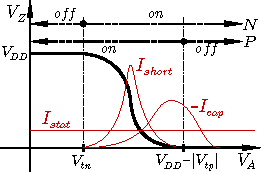
\includegraphics{img/ds/char_inverter.pdf}
	
	\emph{Dynamische Verlustleistung} \qquad \ $P_{dyn} = P_{cap} + P_{short}$\\
	\begin{tabular}{ll}
		\quad Kapazitive Verluste \qquad \ \quad \ & $P_{cap} = \alpha_{01} f C_L V_{DD}^2$\\
		\quad Kurzschlussstrom	& $P_{short} = \alpha_{01} f \beta_n \tau (V_{DD} - 2V_{tn})^3$\\[0.8em]
		\quad Schalthäufigkeit & $\alpha_{0 \rightarrow 1} = \frac{\text{Schaltvorgänge(pos. Flanke)}}{\text{\# Betrachtete Takte}}$\\
		\quad Schalthäufigkeit (periodisch) & $\alpha = \frac{f_\text{switch}}{f_\text{clk}}$\\
	\end{tabular}\\
	Abhängig von den Signalflanken, mit Schaltfunktionen verknüpft\\ 
	$\approx \;$ $V_{DD} 1/\propto $ Schaltzeit: $\frac{V_{DD2}}{V_{DD1}} = \frac{t_{D1}}{t_{D2}}$ (bei Schaltnetzen $t_{log}$)\\
	\textbf{Verzögerungszeit} $\propto$ $\frac{C_Lt_{ox}L_p}{W_p\mu_p\varepsilon(V_{DD} - V_{th})}$
	
	Steigend mit: Kapazitiver Last, Oxiddicke, Kanallänge, Schwellspannung
	
	Sinkend mit: Kanalweite, Ladungsträger Beweglichkeit, Oxyd Dielektrizität, Versorgungsspannung \\ \\
	\emph{Statische Verlustleistung} $P_{stat}$: Sub-Schwellströme, Leckströme, Gate-Ströme
	Abhängigkeit: $V_{DD}\uparrow:P_{stat}\uparrow$ \qquad $V_{th}\uparrow:P_{stat}\downarrow$ \quad (aber nicht proportional)

\section{Volladdierer (VA)/Ripple-C(u)arry-Adder}
\parbox{5.0cm}{ 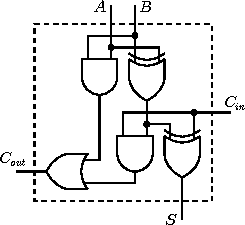
\includegraphics{img/ds/volladdierer.pdf} }
\hspace*{-.7cm}\parbox{5.0cm}{ 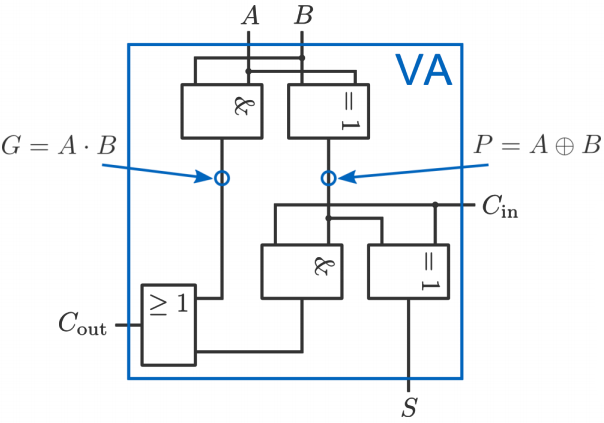
\includegraphics[width=5.0cm]{img/ds/volladdierer-iec.png} } \\
\textbf{Generate} $g_n = a_n \cdot b_n$\\
\textbf{Propagate} $p_n = a_n \oplus b_n$\\
\textbf{Summenbit} $S_n = c_n \oplus p_n= a_n \oplus b_n \oplus c_n$\\
$S_n = \underbrace{a_n\ol{b_n} \ol{c_n} + \ol{a_n}b_n\ol{c_n} + \ol{a_n}\ol{b_n}c_n}_{\text{genau ein Eingang high}} + \underbrace{a_nb_nc_n}_{\text{alle Eingänge high}}$(Ungerade Anzahl von Eingängen 1) \\
\textbf{Carry-out} $c_{n+1} = c_n \cdot p_n + g_n$\\
$c_{n+1}=\underbrace{a_nb_n\ol{c_n} + a_n\ol{b_n}c_n + \ol{a_n}b_nc_n}_{\text{zwei Eingänge 1}} + \underbrace{a_nb_nc_n}_{\text{drei Eingänge 1}}$ (Mindesten zwei Eingänge 1)
\\ \\
\textbf{Laufzeiten} \\
$t_{sn} = \begin{cases} t_{cn} + t_{xor} & t_{cn} > t_{xor} \\ 2 t_{xor} & sonst \end{cases}$\\ \\
$t_{cn+1} = 
\begin{cases}
	t_{and} + t_{or}           & a_n = b_n = 1 \qquad \qquad (g_n=1)   \\
	t_{xor} + t_{and} + t_{or} & a_n = b_n = 0 \qquad \qquad  (p_n = 0, g_n = 0) \\
	t_{cn} + t_{and} + t_{or}  & a_n \ne b_n \qquad \qquad \qquad  (p_n = 1)
\end{cases}$\\

\section{Sequentielle Logik}
Logik mit Gedächtnis (Speicher).
	\subsection{Begriffe/Bedingungen}
	\begin{tabular}{c|l}
	$t_{Setup}$ & Stabilitätszeit vor der aktiven Taktflanke\\
	$t_{hold}$ & Stabilitätszeit nach  der aktiven Taktflanke\\
	$t_{c2q}$ & Eingang wird spätestens nach $t_{c2q}$ am Ausgang verfügbar\\
	 Min. Taktperiode &  $t_{clk} \ge t_{1,c2q} + t_{logic,max} + t_{2,setup}$  \\
	 Max. Taktfrequenz & $f_{max} = \left\lfloor \frac{1}{t_{clk}} \right\rfloor$ \qquad (Nicht aufrunden) \\
	 Holdzeitbedingung & $t_{hold} \le t_{c2q} + t_{logic,min}$  $\ra$ Dummy Gatter einbauen\\
	 Durchsatz & $\frac{1 \text{Sample}}{t_{clk,pipe}} = f$ \\
	 Latenz & $t_{clk} \cdot \#$Pipelinestufen (das zwischen den FFs) \\
	\end{tabular}
	
	
	\subsection{Pipelining} % (fold)
	Nur bei synchronen(taktgesteuerten) Schaltungen möglich!
	\begin{itemize} \itemsep0pt
		\item Aufteilen langer kombinatorischer Pfade durch Einfügen zusätzlicher Registerstufen\\
		$\ra$ Möglichst Halbierung des längsten Pfades
		\item Zeitverhalten beachten (evtl. Dummy-Gatter einfügen)
		\item Durchsatz erhöht sich entsprechend der Steigerung der Taktfrequenz
		\item Gesamtlatenz wird eher größer
		\item Taktfrequenz erhöht sich
	\end{itemize}
	% subsection Pipelining (end)
	
	\subsection{Parallel Processing} % (fold)
	
	Durchsatz = $\frac{\#\text{Modul}}{t_{clk,Modul}} = f$ \qquad \quad Latenz = $t_{clk}$
	\begin{itemize} \itemsep0pt
		\item Paralleles, gleichzeitiges Verwenden mehrere identischer Schaltnetze
		\item Zusätzliche Kontrolllogik nötig (Multiplexer)
		\item Taktfrequenz und Latenz bleiben konstant
		\item Durchsatz steigt mit der Zahl der Verarbeitungseinheiten \\
		ABER: deutlich höherer Ressourcenverbrauch
	\end{itemize}
	% subsection Parallel Processing (end)


\section{Speicherelemente}
	\emph{Flüchtig} Speicherinhalt gehen verloren, wenn Versorgungsspannung $V_{DD}$ wegfällt - Bsp: *RAM\\
	\emph{Nicht Flüchtig} Speicherinhalt bleibt auch ohne $V_{DD}$ erhalten - Bsp: Flash\\
	\emph{Asynchron} Daten werden sofort geschrieben/gelesen.\\
	\emph{Synchron} Daten werden erst mit $clk_{0 \ra 1}$ geschrieben.\\
	\emph{Dynamisch} Ohne Refreshzyklen gehen auch bei angelegter $V_{DD}$ Daten verloren -  Bsp: DRAM\\
	\emph{Statisch} Behält den Zustand bei solange $V_{DD}$ anliegt (keine Refreshzyklen nötig) - Bsp: SRAM\\
	\emph{Bandbreite:} Bitanzahl, die gleichzeitig gelesen/geschrieben werden kann.
	\emph{Latenz:} Zeitverzögerung zwischen Anforderung und Ausgabe von Daten.
	\emph{Zykluszeit:} Minimale Zeitdifferenz zweier Schreib/Lesezugriffe.
	
	\framebox{$\text{Speicherkapazität} = \text{Wortbreite} \cdot 2^\text{Adressbreite}$ }

	\subsection{Speicherzelle/Register}
	Ring aus zwei Invertern.
	
	\subsection{Latch}
	\parbox{5cm}{
		\emph{Set-Reset Latch:} \\ Zwei gegenseitig rückgekoppelte NAND-Gatter. $0$ an R/S schaltet.
		\\	\emph{Enable-Latch:} ändert Speicherzustand auf $D$ nur wenn $e=1$
	}
	\parbox{.5cm}{\ }
	\parbox{2cm}{
		\begin{tabular}{c|c} e & Q \\ \hline 0 & Q \\ 1 & D \end{tabular}
	}
	

	\subsection{Flip-Flop}
		\parbox{5cm}{
			Besteht aus zwei enable-Latches \\
			\emph{Flip-Flop:} Ändert Zustand bei steigender/(fallender) Taktflanke.\\
		}
		\parbox{.5cm}{\ }
		\parbox{2cm}{
			\begin{tabular}{c|c|c} clk & $Q$ & $\ol Q$ \\ \hline $0 \ra 1$ & $D$ & $\ol D$ \\ sonst & $Q$ & $\ol Q$ \end{tabular}
		}


\section{Automaten} % (fold)

DFA 6-Tupel $\eset{I, O, S, R, f, g}$ \\

\begin{tabular}{r | l} 
$I$ & Eingabealphabet \\
$O$ &  Ausgabealphabet \\
$S$ & Menge von Zuständen \\
$R \subseteq S$ &  Menge der Anfangszustände \\
$f: S \times I \ra S$  &  Übergangsrelation \\
$g$ & Ausgaberelation \\
\end{tabular}

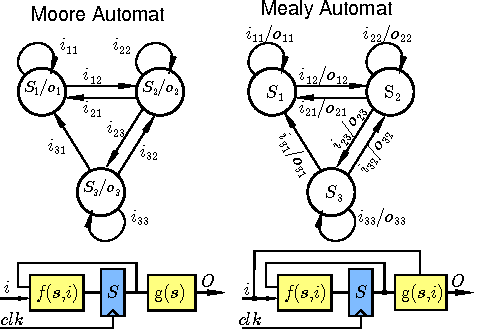
\includegraphics{img/ds/automaten.pdf}\\


\begin{tabular}{c | c}
 Moore & Mealy \\ \hline
 Ouput hängt nur vom Zustand ab & Output hängt von Zustand und Eingabe ab\\
 $s'=f(s,i)$, $o=g(s)$ &  $s'=f(s,i)$, $o=g(s,i)$ \\
 $g: S \ra O$ & $g: S \times I \ra O$
\end{tabular}

\begin{multicols}{2}
\noindent\textbf{Vorteile}
\begin{itemize} \itemsep0pt
 \item Kein kombinatorischer Pfad von Eingängen zu Ausgängen
 \item Wichtig für Begrenzung der Logiktiefe in sequentiellen Schaltwerken, insb. bei Verkettung
\end{itemize}
\textbf{Nachteile}
\begin{itemize} \itemsep0pt
 \item Hohe Anzahl an Zuständen
\end{itemize}
\pagebreak
\textbf{Vorteile}
\begin{itemize} \itemsep0pt
 \item Weniger Zustände
 \item Übersichtliche Beschreibung
 \item Allgemeinster Fall einer FSM
\end{itemize}
\textbf{Nachteile}
\begin{itemize} \itemsep0pt
 \item Lange kombinatorische Pfade bei Verkettung
 \item in der Praxis zu vermeiden
\end{itemize}


\end{multicols}

% subsection Vorgehensweise (end)

% Ende der Spalten
\end{multicols*}
% Dokumentende
% ======================================================================
\end{document}
